\documentclass[crop,tikz]{standalone}% 'crop' is the default for v1.0, before it was 'preview'
%\usetikzlibrary{...}% tikz package already loaded by 'tikz' option
\begin{document}
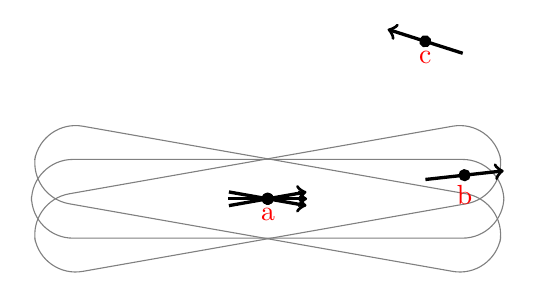
\begin{tikzpicture}[remember picture,shift=(current page.center)]
    \begin{scope}[rotate=10]
    \draw[rounded corners=15pt,gray]
  (-3,-0.5) rectangle ++(6,1);
  \filldraw[black] (0,0) circle (2pt) node[anchor=north,red]{a};
  \draw[->,very thick] (-0.5,0) -- (0.5,0);
  \end{scope}
  
  
  \begin{scope}[rotate=0]
    \draw[rounded corners=15pt,gray]
  (-3,-0.5) rectangle ++(6,1);
  \filldraw[black] (0,0) circle (2pt);
  \draw[->,very thick] (-0.5,0) -- (0.5,0);
  \end{scope}
  
  
  \begin{scope}[rotate=-10]
    \draw[rounded corners=15pt,gray]
  (-3,-0.5) rectangle ++(6,1);
  \filldraw[black] (0,0) circle (2pt);
  \draw[->,very thick] (-0.5,0) -- (0.5,0);
  \end{scope}
  
  
  \begin{scope}[shift={(2.5, 0.3)}]
    \begin{scope}[rotate=4]
    \filldraw[black] (0,0) circle (2pt) node[anchor=north,red]{b};
    \draw[->, very thick] (-0.5,-0.02) -- (0.5,0.02);
    \end{scope}
  \end{scope}
  %
  \begin{scope}[shift={(2, 2)}]
    \begin{scope}[rotate=160]
    \filldraw[black] (0,0) circle (2pt) node[anchor=north,red]{c};
    \draw[->, very thick] (-0.5,-0.02) -- (0.5,0.02);
    \end{scope}
  \end{scope}
\end{tikzpicture}

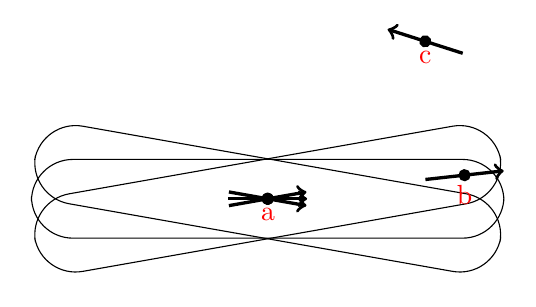
\begin{tikzpicture}[remember picture,shift=(current page.center)]
    \begin{scope}[rotate=10]
    \draw[rounded corners=15pt]
  (-3,-0.5) rectangle ++(6,1);
  \filldraw[black] (0,0) circle (2pt) node[anchor=north,red]{a};
  \draw[->,very thick] (-0.5,0) -- (0.5,0);
  \end{scope}
  
  
  \begin{scope}[rotate=0]
    \draw[rounded corners=15pt]
  (-3,-0.5) rectangle ++(6,1);
  \filldraw[black] (0,0) circle (2pt);
  \draw[->,very thick] (-0.5,0) -- (0.5,0);
  \end{scope}
  
  
  \begin{scope}[rotate=-10]
    \draw[rounded corners=15pt]
  (-3,-0.5) rectangle ++(6,1);
  \filldraw[black] (0,0) circle (2pt);
  \draw[->,very thick] (-0.5,0) -- (0.5,0);
  \end{scope}
  
  
  \begin{scope}[shift={(2.5, 0.3)}]
    \begin{scope}[rotate=4]
    \filldraw[black] (0,0) circle (2pt) node[anchor=north,red]{b};
    \draw[->, very thick] (-0.5,-0.02) -- (0.5,0.02);
    \end{scope}
  \end{scope}
  %
  \begin{scope}[shift={(2, 2)}]
    \begin{scope}[rotate=160]
    \filldraw[black] (0,0) circle (2pt) node[anchor=north,red]{c};
    \draw[->, very thick] (-0.5,-0.02) -- (0.5,0.02);
    \end{scope}
  \end{scope}
\end{tikzpicture}
\end{document}
